% !TEX encoding = UTF-8
\documentclass{beamer}
\usepackage[T1]{fontenc}
\usepackage[utf8]{inputenc}
\usepackage[english]{babel}
\usepackage{graphicx}
\graphicspath{{img/}}

\title{GIT - Two word introduction}
\author{Luigi Capogrosso \and Jasin Atipi}
\usetheme{CambridgeUS}

\begin{document}

\begin{frame}
\maketitle
\end{frame}

\begin{frame}
\frametitle{What is version control?}
\begin{itemize}
\item <1-> Version control is a tool that allows you to...
\item <2-> \textbf{Collaborate} \\ 
Creating anything with other people, from academic papers to entire websites and application
\item <3-> \textbf{Track and revert changes} \\ 
Mistakes happen. Wouldn't it be nice if you could see the changes that have been made and then go back in time to fix something that went wrong?
\end{itemize}
\end{frame}

\begin{frame}
\frametitle{Why Git?}
\begin{itemize}
\item<1-> \textbf{Fast!} Access information quickly and efficiently
\item<2-> \textbf{Distributed!} Everyone has their own local copy
\item<3-> \textbf{Scalable!} Enables potentially thousands (millions!) of developers to work on a single project
\item<4-> \textbf{Branches!} Keep your coding experiments separate from code that is already working
\item<5-> Every one has a local copy of the \textbf{shared files} and the \textbf{history}
\end{itemize}
\end{frame}

\begin{frame}
\frametitle{Git has its own vocabulary}
\begin{itemize}
\item <1-> A \textbf{repository} is where you keep all the files you want to track
\item <2-> A \textbf{branch} is the name for a separate line of development, with its own history
\item <3-> A \textbf{commit} is an object that holds information about a particular change
\end{itemize}
\end{frame}

\begin{frame}
\frametitle{GitHub}
\begin{itemize}
\item Online git repository
\item Free for open source projects
\end{itemize}
\begin{figure}
\centering

\includegraphics[height=3.5cm, width=4.5cm]{github_logo}
\end{figure}
\end{frame}

\begin{frame}[fragile]
\frametitle{Basics}
\begin{itemize}
\item \verb!git clone $url! \\ 
copy the whole repository and its history on the local machine
\end{itemize}
\begin{figure}
\centering
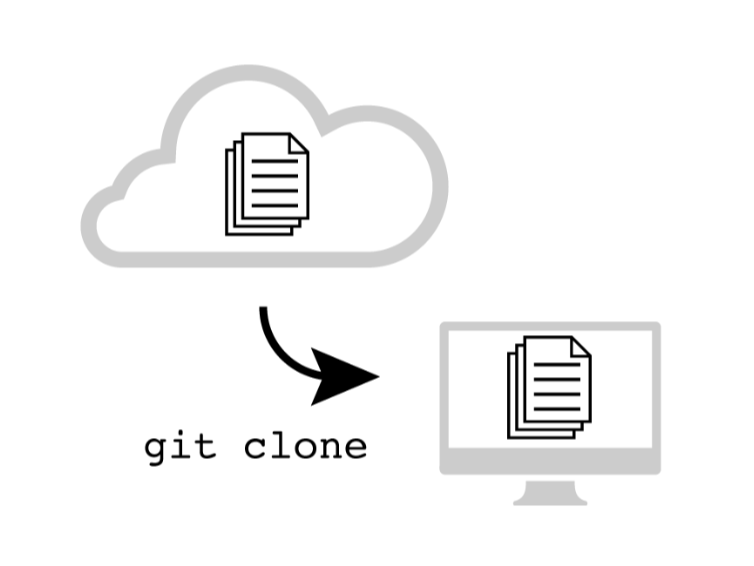
\includegraphics[height=3.5cm, width=4.5cm]{clone}
\end{figure}
\end{frame}

\begin{frame}[fragile]
\frametitle{Basics}
\begin{itemize}
\item \verb!git add $file! 
\item \verb!git commit -m "$message"! \\ 
the new release is confirmed and locked in the local repository
\end{itemize}
\begin{figure}
\centering
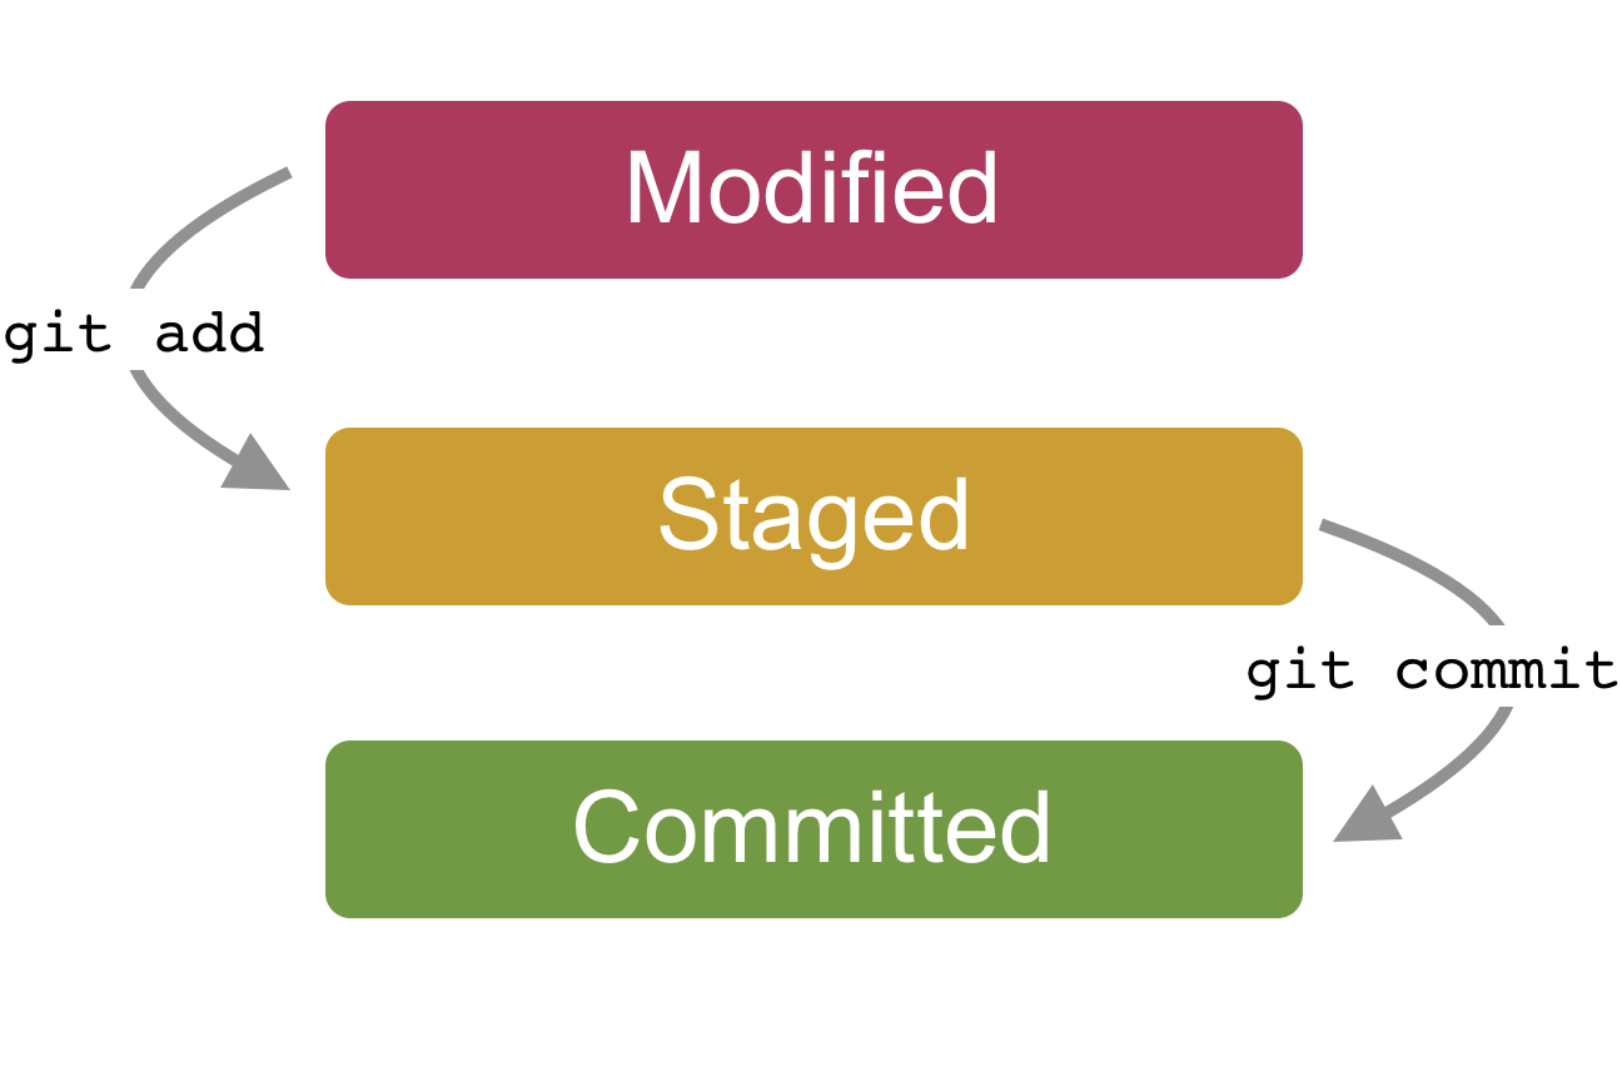
\includegraphics[height=3.5cm, width=4.5cm]{commit}
\end{figure}
\end{frame}

\begin{frame}[fragile]
\frametitle{Basics}
\begin{itemize}
\item \verb!git push! \\ 
sends the committed files to the remote repository
\end{itemize}
\begin{figure}
\centering
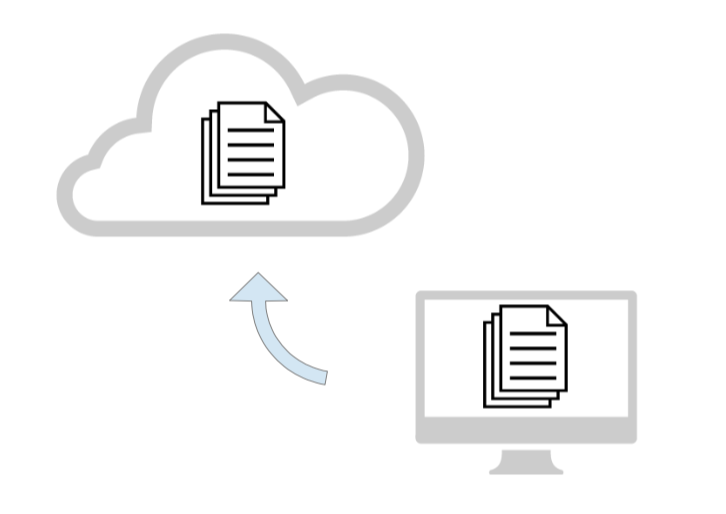
\includegraphics[height=3.5cm, width=4.5cm]{push}
\end{figure}
\end{frame}

\begin{frame}[fragile]
\frametitle{Basics}
\begin{itemize}
\item \verb!git pull! \\ 
downloads the updated files from the remote repository
\end{itemize}
\begin{figure}
\centering
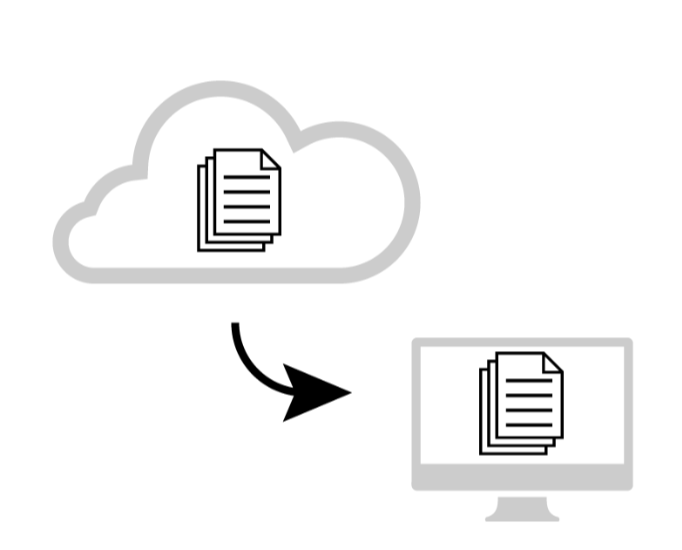
\includegraphics[height=3.5cm, width=4.5cm]{pull}
\end{figure}
\end{frame}

\begin{frame}[fragile]
\frametitle{Basics}
\begin{itemize}
\item \verb!git branch! \\ 
list all available branches
\end{itemize}
\begin{figure}
\centering
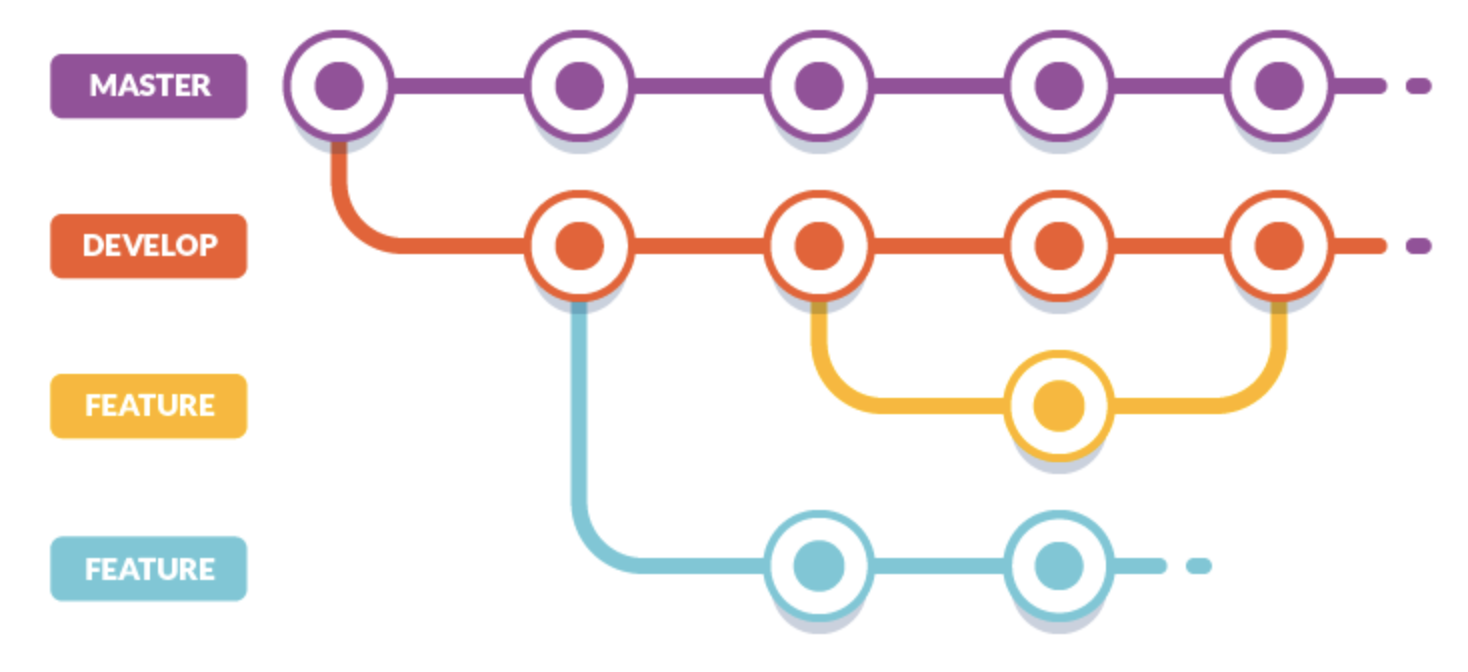
\includegraphics[height=3.5cm, width=7cm]{branching}
\end{figure}
\end{frame}

\begin{frame}[fragile]
\frametitle{Basics}
\begin{itemize}
\item \verb!git checkout $branchname! \\ 
switch from the current branch to \verb!$branchname!
\end{itemize}
\end{frame}

\begin{frame}[fragile]
\frametitle{Questions?}
\begin{figure}
\centering
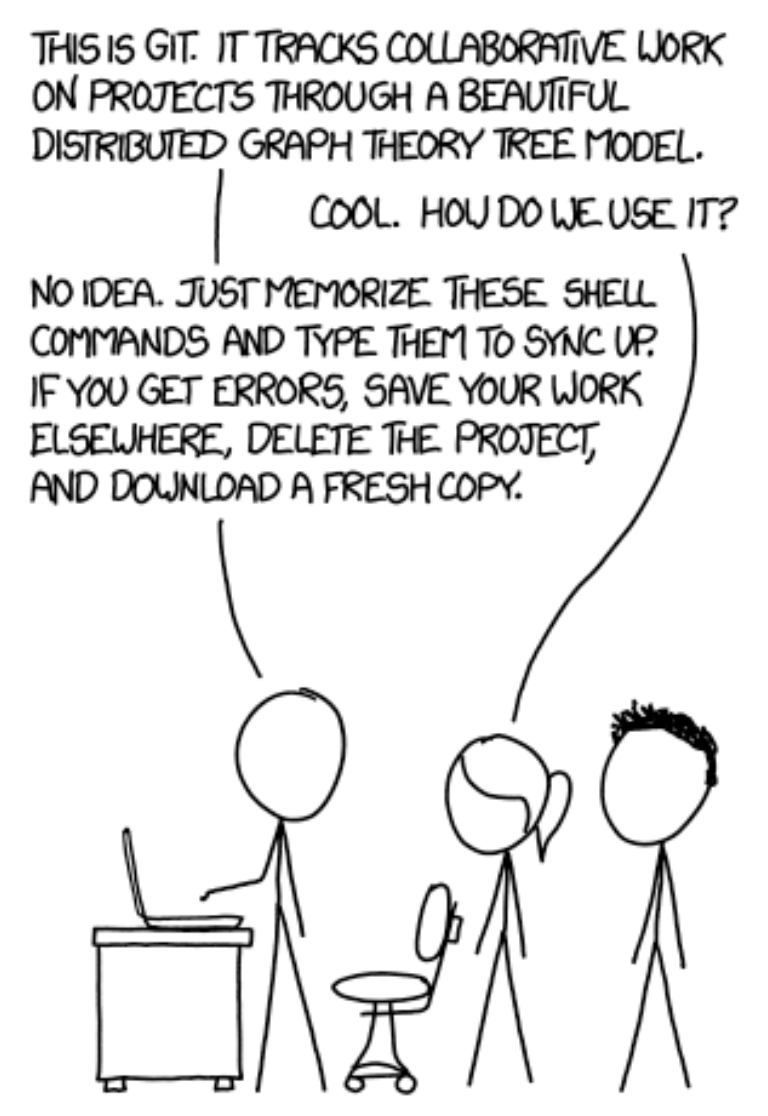
\includegraphics[height=7cm, width=4.5cm]{questions}
\end{figure}
\end{frame}

\end{document}